%!TEX root = Thesis_main.tex

\chapter{Results}
\label{chapter7}
\section{Simulations results}
\begin{floatingfigure}[r]{.33\textwidth}
	\centering
	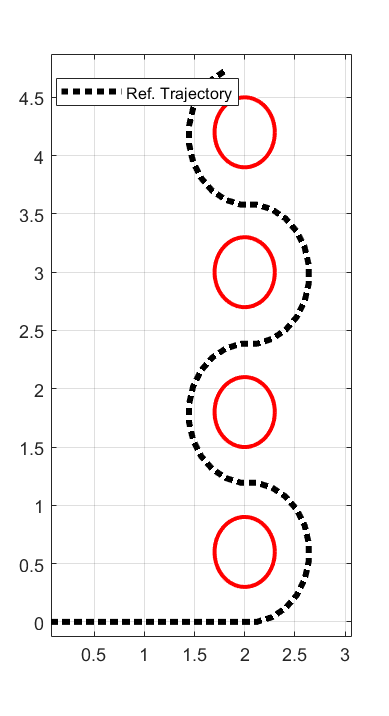
\includegraphics[scale=0.4]{traj_base_curves}
	\caption{Base trajectory for simulations: radius of the curve = 0.6m\label{traj_base_curves}}
\end{floatingfigure}
The goal of the initial simulations is to assess the actual convenience of our approach and to tune the MPC parameters and weights. Once achieved good performances with a proper set of parameters, the controller can be tested with the physical system.\\
Initially some simulations with only the mobile base have been run on a trajectory with low-radius curves (in Figure \ref{traj_base_curves}), seeing the effect of different control horizon lengths and of input disturbances. This trajectory has been chosen to simulate how our controller tracks a trajectory which goes around some obstacles. No obstacle avoidance is considered in this simulation.
\begin{figure}[!h]
	\centering
	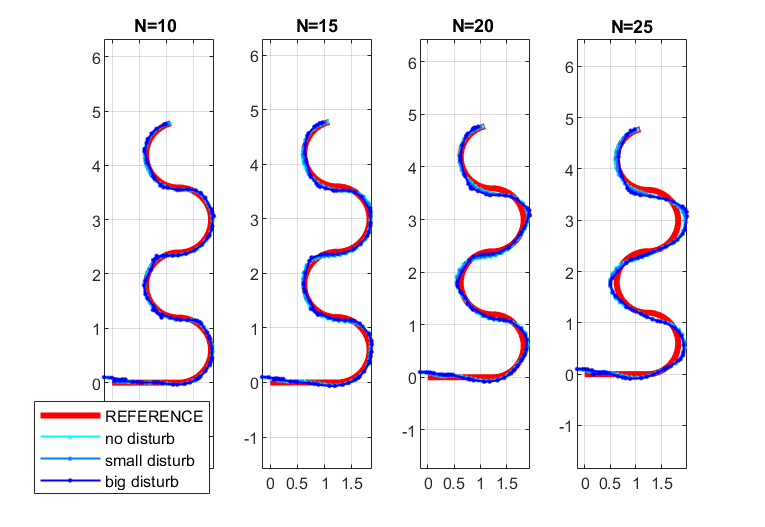
\includegraphics[scale=0.5]{base_curves}
	\caption{Mobile platform trajectories with different N}
	\label{base_curves}
\end{figure}
\begin{figure}[!h]
	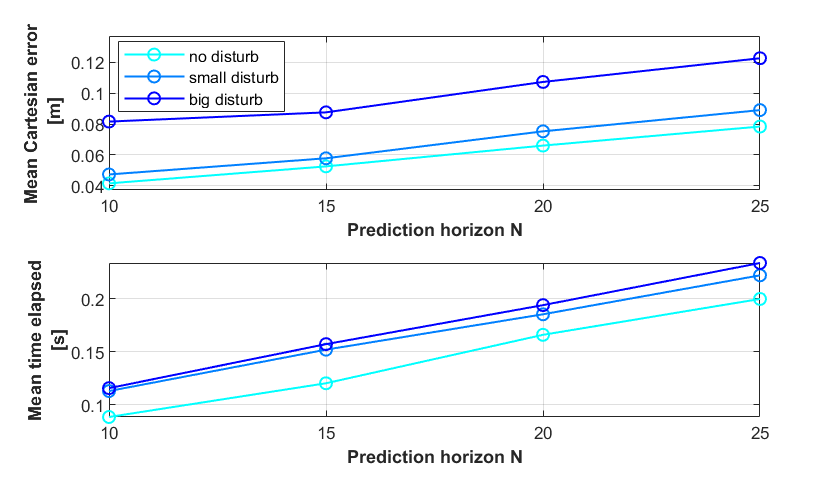
\includegraphics[scale=0.5]{base_curves_error}
	\centering
	\caption{Cartesian error and Optimization time when varying N}
	\label{base_curves_errors}
\end{figure}
\\In Figure \ref{base_curves} the trajectories that the mobile base follows are shown, considering different levels of random disturbances added to the input commands and considering different values of $N$. In Figure \ref{base_curves_errors} the relative errors and optimization times are shown. From these results we can notice that our controller is able to manage even high disturbances, but because of the limitation introduced by the parameterization of the input, it is more difficult for the optimizer to find a curve built on polynomial input commands that correctly approximates the given trajectory. This effect is even enlarged by the weighting profile of the cost function which give less importance to the accuracy of the first steps in the control horizon. Nevertheless Figure \ref{base_curves_errors} let us see that the time elapsed during the the optimization process doesn't increase exponentially like in traditional MPC, but it has just a slight increment.\\
\begin{figure}[!h]
	\centering
	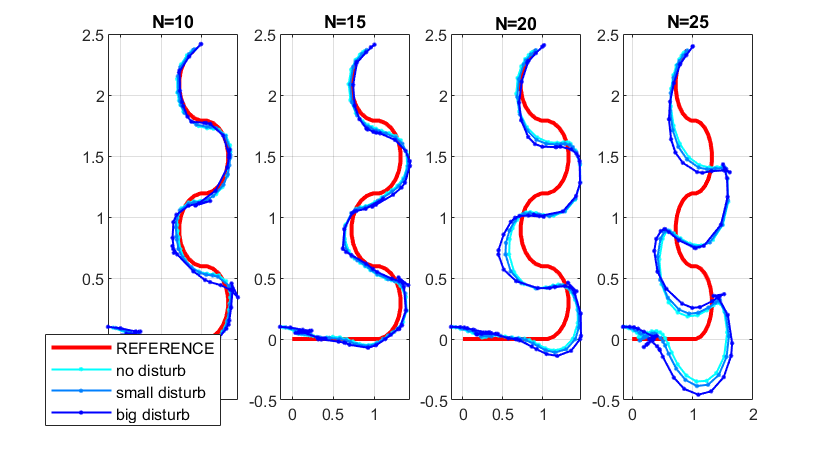
\includegraphics[scale=0.5]{base_curves2}
	\caption{Mobile platform trajectories with different N with a small-radius trajectory}
	\label{base_curves2}
\end{figure}
\begin{figure}[!h]
	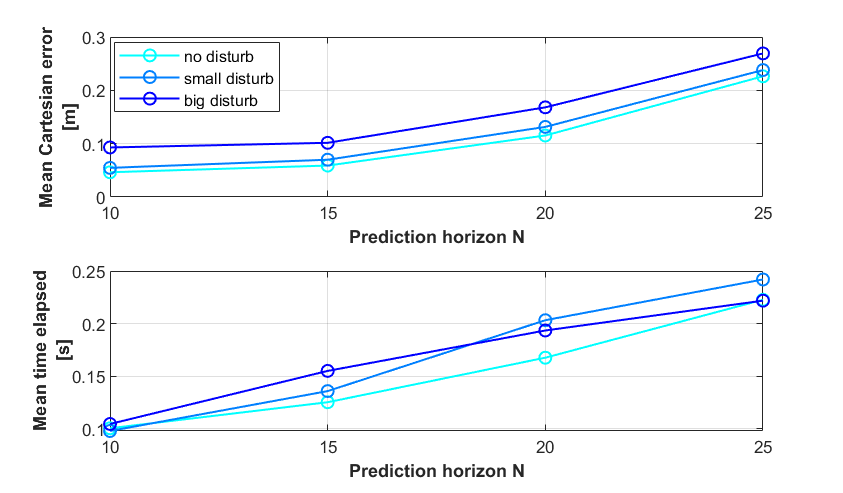
\includegraphics[scale=0.5]{base_curves_error2}
	\centering
	\caption{Cartesian error and Optimization time when varying N with a small-radius trajectory}
	\label{base_curves_errors2}
\end{figure}
To better understand the effect of a too high $N$ for complex trajectories, the same experiment has been run with a very similar trajectory but with a radius of the curves of $0.3$m instead of $0.6$m. The results of the simulations are found in Figures \ref{base_curves2} and \ref{base_curves_errors2}, where the effect of increasing $N$ is even more evident.
\begin{figure}[h!]
	\centering
	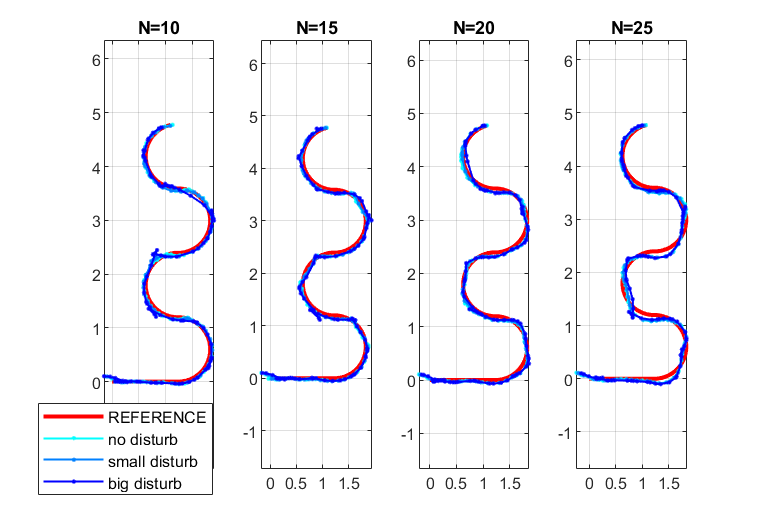
\includegraphics[scale=0.5]{base_curves3}
	\caption{Mobile platform trajectories with different N using 5th order polynomial inputs}
	\label{base_curves3}
\end{figure}
\begin{figure}[h!]
	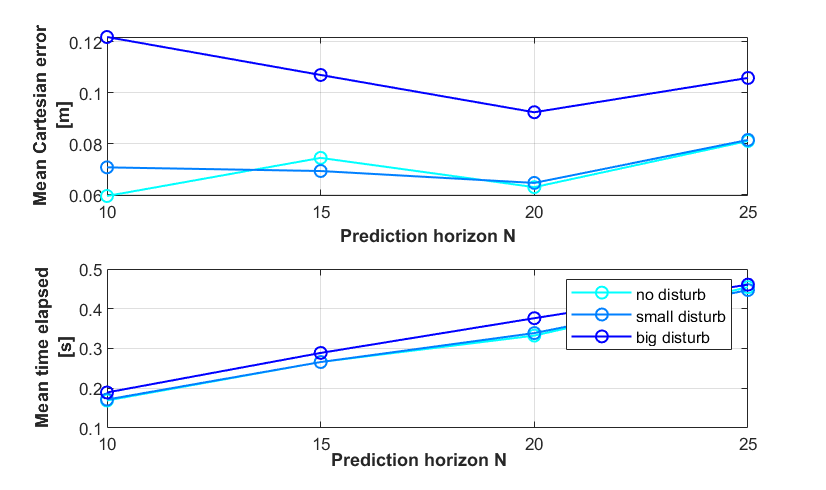
\includegraphics[scale=0.5]{base_curves_error3}
	\centering
	\caption{Cartesian error and Optimization time when varying N using 5th order polynomial inputs}
	\label{base_curves_errors3}
\end{figure}
\begin{figure}[h!]
	\centering
	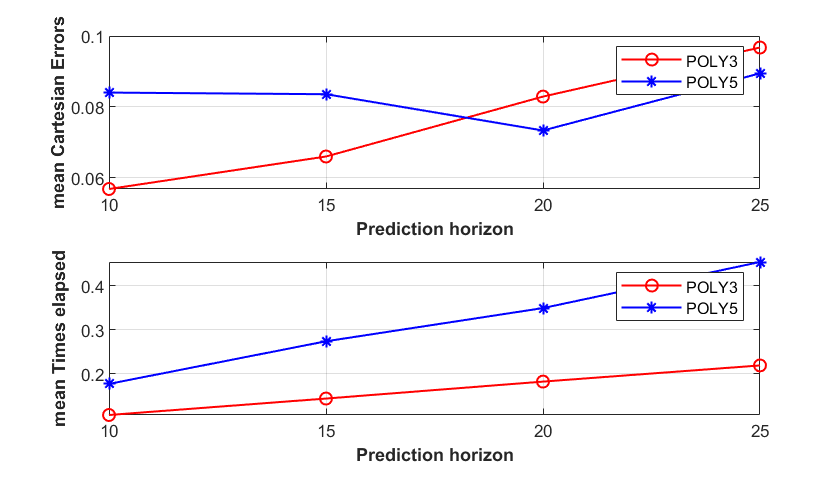
\includegraphics[scale=0.5]{base_curves_poly5}
	\caption{Comparison of errors and time of computation for 3rd and 5th order polynomial inputs}
	\label{base_curves_poly5}
\end{figure}
The previous tests have been performed describing the input commands $v$ and $\omega$ with a 3rd order polynomial. As Figures \ref{base_curves3} and \ref{base_curves_errors3} show, the effect of $N$ is lowered increasing the order of the input polynomial to 5. In Figure \ref{base_curves_poly5} a comparison between the two parameterizations in term of Cartesian error and elapsed times is shown; as was foreseeable, since the unknowns of the problem are more numerous having increased the polynomial order, the time needed for the computation of the optimization problem is higher. On the other hand, lower errors were expected with higher order polynomials; however a better performance in this sense is reached only at high $N$, since the optimizer can now found trajectories which stay closer to the reference trajectory.
\\\\
\begin{figure}[h!]
	\centering
	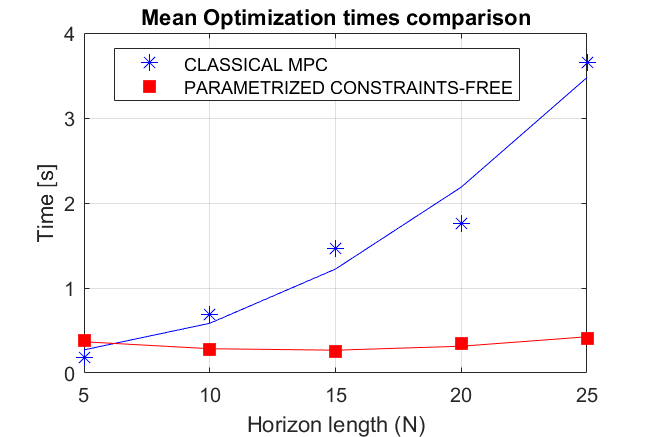
\includegraphics[scale=0.60]{solving_times_small}
	\caption{Solving time comparison}
	\label{solving_times}
\end{figure}
Once understood how some parameters affect the performance of the controlled system, we assessed the actual convenience of the presented approach running some simulations with the entire Mobile Manipulator system. We compared the solving times of our approach with the ones of a traditional MPC at different time horizon tracking a simple sinusoidal trajectory for the end effector position, in Figure \ref{solving_times}. It is easy to see the convenience of our approach, since the number of the unknowns that the optimizer has to find does not increase with $N$ and so with the dimension of the problem. In other words, the mean time needed to the optimizer to solve the MPC problem stays almost constant instead of increasing exponentially.\\
The following results have been obtained simulating the control of the Mobile Manipulator performing two types of motion, handling and grasping, since the controller is meant to be suitable for all the phases of a pick-and-transport task. The stage costs used in both cases have been explained in Chapter \ref{chapter6}.
\subsection{Mobile Manipulator Handling Simulations}
The entire Mobile Manipulator has been simulated performing a trajectory tracking in joint space, i.e. a custom trajectory for each coordinate of the base and for each manipulator joint has been given. Typically, in Mobile Manipulator handling tasks, the main objective is the locomotion of the base, while the arm can be kept stationary. For this reason a constant trajectory is asked to be tracked for the joints of the arm, while we have chosen to give the mobile base a trajectory involving high velocities to track. The results of the simulations are shown in Figures \ref{handling_traj} and \ref{handling_joints}. 
\begin{figure}[p]
	\centering
	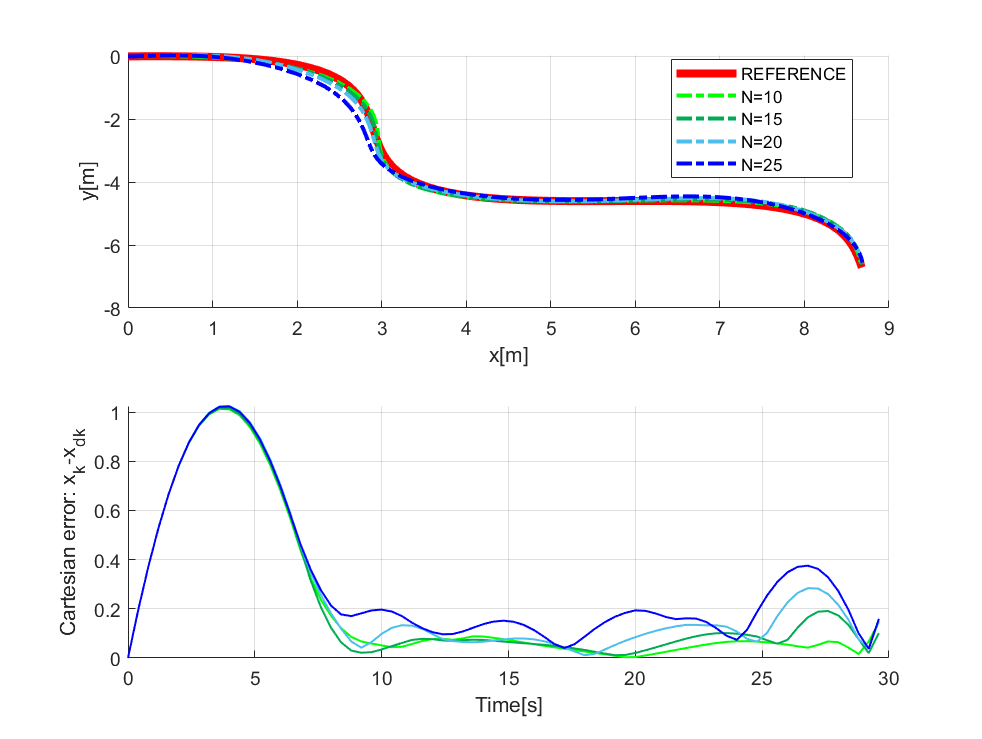
\includegraphics[scale=0.45]{handling_traj}
	\caption{Trajectory following of the mobile base during a Mobile Manipulator handling task}
	\label{handling_traj}
\end{figure}
\begin{figure}[p]
	\centering
	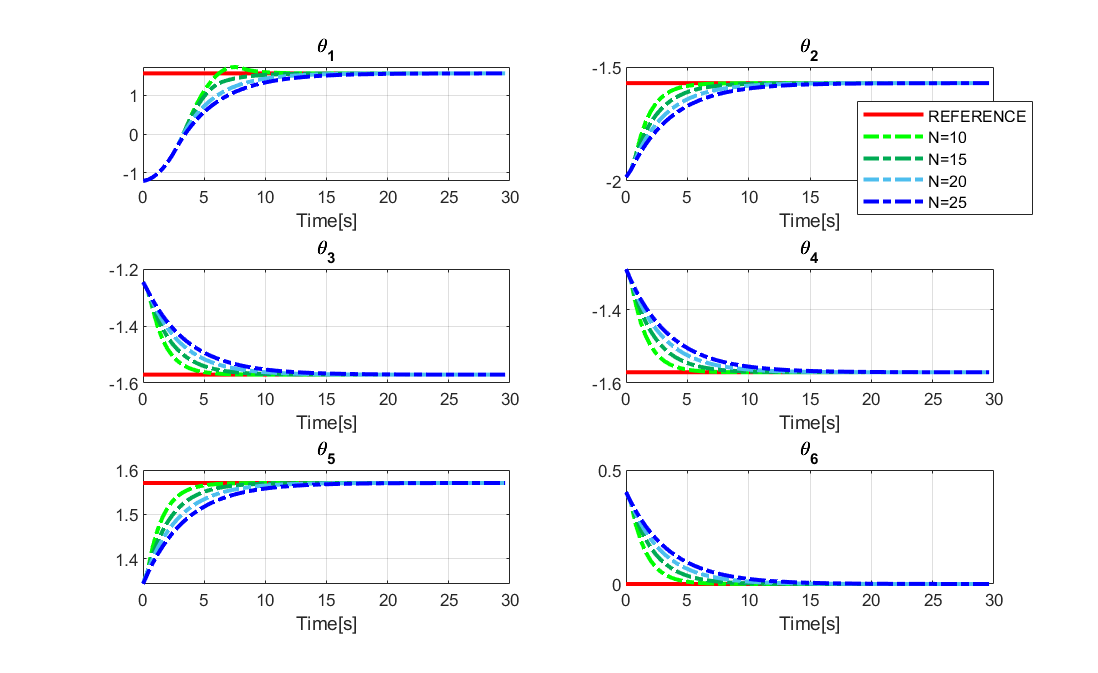
\includegraphics[scale=0.45]{handling_joints}
	\caption{Trajectory following of the joints during a Mobile Manipulator handling task}
	\label{handling_joints}
\end{figure}
A first consideration can be done on the Cartesian errors in tracking the mobile base motion. Indeed, in Figure \ref{handling_traj}, a peak of $1$ m of error can be seen at the very beginning of the trajectory. This is because the reference trajectory does not start with velocity equal to zero, while the robot starts from a stationary position; for this reason we can notice that the robot cuts the corner of the path to keep up with the reference trajectory. This "cutting the corner", actually, is the reason why increasing $N$, the errors in tracking the base position increase, as can also be seen in Figure \ref{handling_traj}. A second consideration is done on the trajectory tracking of the joint variables. Figure \ref{handling_joints} shows that our controller tracks very well a constant reference trajectory, varying the convergence to the constant value depending on $N$. This is because, even without imposing a constraint on the terminal state, our controller is driven to track exactly the reference value at the end of the prediction horizon; having kept the time step $T$ constant in all the simulations, a smaller time horizon leads to more reactive responses of the state.

\subsection{Mobile Manipulator Grasping Simulations}
The entire Mobile Manipulator has then been simulated performing an EE position and orientation trajectory tracking on a sinusoidal 3D path. Since part of the trajectory lies outside the UR5 workspace, the Mobile Manipulator is asked to move in a synchronized fashion to correctly track the end effector pose. 
\begin{figure}[h!]
	\centering
	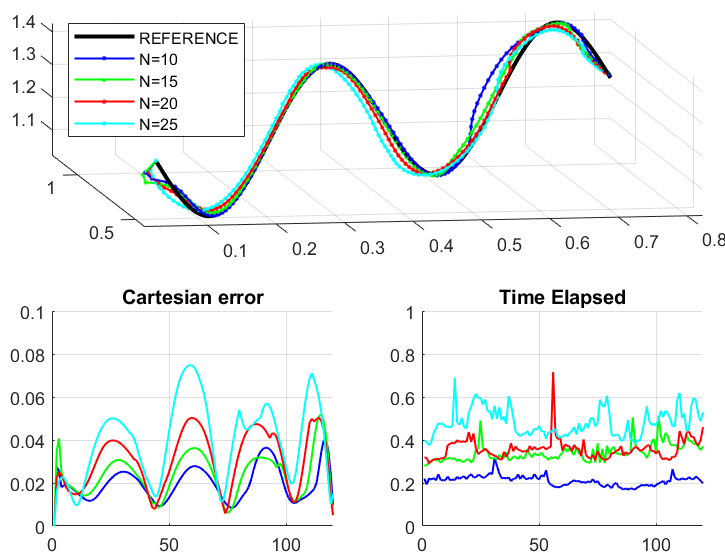
\includegraphics[scale=0.55]{end_effector_tests}
	\caption{End effector pose trajectory following with different N }
	\label{end_effector_tests}
\end{figure}
Results of these simulations are showed in Figure \ref{end_effector_tests}. The considerations made about previous tests still stand: the biggest limit of this controller is that it cannot find a trajectory defined with polynomial inputs that can stay close to too complex desired trajectories during long prediction horizons. The same effect has been seen keeping constant $N$ and increasing the time step $T$. Nonetheless, also in these results, it is possible to see how the optimization time has just a slight increment increasing $N$.


\paragraph{simulation self collision}
\paragraph{control actions}

\fix{passaggio da una funz costo all'altra?}

%%%%%%%%%% ---------------------

\section{Physical experiments results}
	\fix{parlare del fatto che gli esperimenti sono stati fatti a basse velocità per diversi motivi: software e del posizionamento della base che non funziona bene ad alte velocità e si possono mettere anche dei grafici per la ripetibilità della base e una foto.
	Parlare del sistema di telecamere che è stato usato ma non funzionava bene in termini di stabilità e magari mettere qualche foto?}

	\subsection{Movement of the system toward grasping area}


\subsection{Trajectory tracking in grasping operation}

The controller has been tested to perform grasping operations tracking EE trajectories as position and orientation in time as well as a desired motion of the base. For these experiments the system shows a response comparable to the model used in simulation. Anyway, considering the errors due to the positioning system of the base as mentioned before, did not allow to test the system at high speed. The time chosen to perform this task has been setted between $35$ and $45 s$ according to the choice of $T$. 


	\begin{table}[]
	
	\centering

	\begin{tabular}{|l|l|l|ll}
	\cline{1-2}
	\multicolumn{2}{|l|}{ \textbf{Parameters} }	\\ \cline{1-2}
	$N$     				&  $10$ 	      					\\ \cline{1-2}
	$T$     				&  $0.4\ s$  	      					\\ \cline{1-2}
	$b$     				&  $3$ 	      						\\ \cline{1-2}
	$w_1$    				&  $1e6$       						\\ \cline{1-2}
	$w_2$    				&  $50$       						\\ \cline{1-2}
	$w_3$    				&  $1e5$       						\\ \cline{1-2}
	$w_4$    				&  $5e3$       						\\ \cline{1-2}
	$w_5$    				&  $0$      						\\ \cline{1-2}
	\end{tabular}
	\quad
	\begin{tabular}{|l|l|l|ll}
	\cline{1-3}
	\textbf{Constraints}    	& \textbf{min} 					& \textbf{max}			\\ \cline{1-3}
	$x_b$		 			 		&  -0.15 $m$ 					&  3.00 $m$ 			\\ \cline{1-3}
	$y_b$		 			 		&  -2.60 $m$ 					&  0.20 $m$ 			\\ \cline{1-3}
	$\theta_b$ 			 		&  -$\infty$  					&  +$\infty$ 			\\ \cline{1-3}
	$\Theta_1$ (Base)			&  -350°  						&  350° 				\\ \cline{1-3}
	$\Theta_2$ (Shoulder)		&  -180° 						&  0°		 			\\ \cline{1-3}
	$\Theta_3$ (Elbow) 			&  -140° 						&  140°		 			\\ \cline{1-3}
	$\Theta_4$ (Wrist1) 		&  -180° 						&  0°		 			\\ \cline{1-3}
	$\Theta_5$ (Wrist2)			&  -140° 						&  97°		 			\\ \cline{1-3} 
	$\Theta_6$ (Wrist3) 		&  -357° 						&  357°		 			\\ \cline{1-3}
	$\dot{v}$ 			 		&  -0.1 $m/s^2$					&  -0.1 $m/s^2$ 		\\ \cline{1-3}
	$\dot{\omega}$		 		&  -0.1 $rad/s^2$ 				&  -0.1 $rad/s^2$		\\ \cline{1-3}
	$\dot{\Theta}_{1,\dots,6}$	&  -0.2 $rad/s$					&  -0.2 $rad/s$ 		\\ \cline{1-3}
	\end{tabular}
	\caption{Experiment Parameters}
	\label{tableparam1}
	\end{table}


	\fix{NON SO SE QUESTO riusciamo a farlo, occhio! Nel caso se si riesce mettiamo nei grafici una comparison (se ne vale la pena) ... 
	Parameterization has been chosen as in simulation, so comparing linear and constant parameterization for the arm joints.} The gripper used in the experiments is a Robotiq 2-Finger 85mm for Universal Robots. The instant at which the gripper has to be closed was defined offline and the communication ensured through a ROS node. The first experiment's results, performed with a linear parameterization for the arm joints are obtained using the parameters shown in Table \ref{tableparam1}. 
	In Figure \ref{traj_ee1} the performed trajectory is shown in a 3D graph. 
	\begin{figure}[h!]
	\centering
	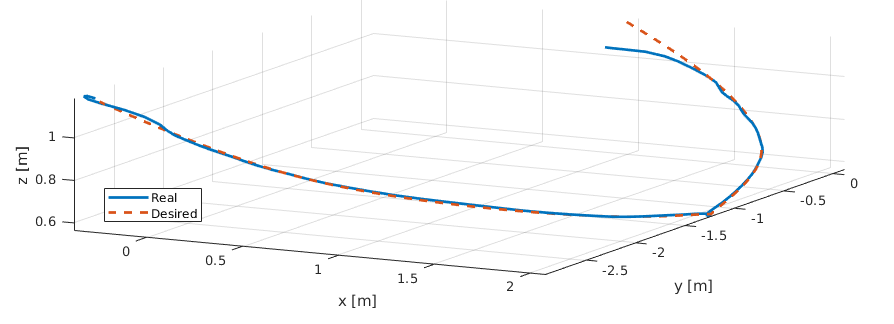
\includegraphics[scale=0.36]{traj_ee1.png}
	\caption{EE position during grasping}
	\label{traj_ee1}
	\end{figure}

	The results are then compared in Figure \ref{traj_ee1_comp} with the trajectory performed in simulation. The position and orientation of the EE are measured through the positioning system of the base presented in \ref{chapter6} and then using forward kinematics to compute position of the end effector. 

	\begin{figure}[h!]
	\centering
	
\includegraphics[scale=0.2]{empty}
	\caption{EE position comparison during grasping}
	\label{traj_ee1_comp}
	\end{figure}
	The trajectories in \ref{traj_ee1_comp} show that the system behaviour is close to the simulated one, this confirm the accuracy of the model. We will now analize the errors in performing this trajectory with respect to the desired one.  

	Given that we are interested in a tracking problem, i.e. the system has to be in the correct position at the right instant, and that the controller works at a fixed frequency $f_c=\frac{1}{T}$, the number of the given points $x_d$ implies that we are referring to a trajectory and not to a path. For this reason the offline planned trajectory has to be generate according to that. 
	In Figure \ref{error_xyz1} absolute errors in $x$,$y$ and $z$ position of the EE is shown for a linear parameterization of the arm joints velocities.

	\begin{figure}[h!]
	\centering
	
\includegraphics[scale=0.2]{empty}
	\caption{EE position errors during grasping}
	\label{error_xyz1}
	\end{figure}
	\begin{figure}[h!]
	\centering
	
\includegraphics[scale=0.2]{empty}
	\caption{EE orientation errors during grasping}
	\label{error_orient1}
	\end{figure}

	Errors in orientation are shown in Figure \ref{error_orient1}. Orientation is important in grasping operation because trajectories have to be planned according to the part to be handled. What is possible to see is that the more the points are close eachother  

